\scanpage{306}
\margin{\deleted{$\unsure{\varphi}$}\quad $\unsure{\xi|6}$}
$X\times Y\longrightarrow Y$ morphisme de schémas algébriques \inserted{(intègres sur $k$ alg clos)}

$D$ diviseur sur $Y$

\uline{Supposons} que pour tt $x\in X(k)$ on ait
\[
\unsure{\varepsilon_x}\; x.D-D\quad\text{lin. équivalent \unsure{à|:}}\quad0
\]
C'est le cas si $X$ \inserted{ou $Y$} est ``d'irrégularité nulle'' et $\exists e\in X$ qui opère trivialement sur $Y$. \deleted{\unsure{C'est bien entendu}}

\deleted{$\unsure{\Rightarrow}$}
\uline{Alors} \deleted{l'ens des $xD$} On peut trouver un \deleted{\unsure{espace projectif} $P$ \unsure{avec famille de dim finie|avec la famille de dim finie}} \deleted{famille linéaire} \inserted{système linéaire} borné $P$ de diviseurs sur $Y$, contenant $D$ et un morphisme $X\times P\longrightarrow P$, qui ensemblistement correspond à : $(x,D)\longrightarrow x.D$.
\figure{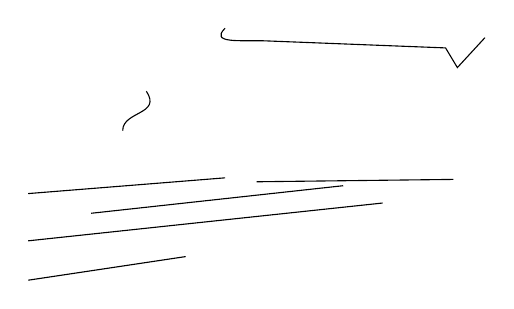
\begin{tikzpicture}[x=1cm,y=1cm]
\draw (2.5,2.6)..controls (2.3,2.4) and (2.7,2.45)..(3,2.44)--(5.3,2.35)--(5.45,2.1)--(5.8,2.48);
\draw (1.2,1.3)..controls (1.2,1.55) and (1.7,1.5)..(1.5,1.8);
\draw (0,.5)--(2.5,.7) (0.8,.25)--(4,.6) (2.9,.65)--(5.4,.68) (0,-.1)--(4.5,.38) (0,-.6)--(2,-.3);
\end{tikzpicture}}
\mspage{305}
